\section{Path of a light ray}

To determine the projection of a light ray as it passes through a lens at any given position, the following steps can be followed:
\begin{enumerate}
    \item Draw a line parallel to the chosen ray, passing through the center of the lens. 
    \item Identify the intersection point of this line with the focal plane.
    \item The ray will travel from the point where it crosses the lens to the point located on the focal plane.
\end{enumerate}
\begin{figure}[H]
    \centering
    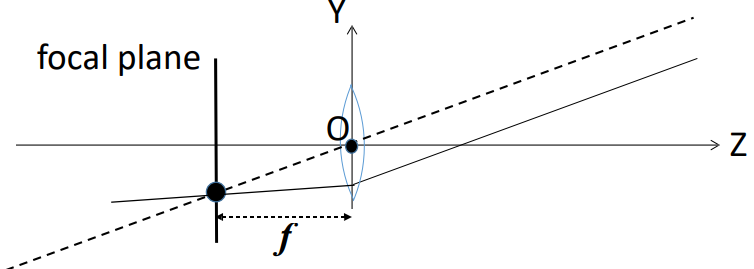
\includegraphics[width=0.4\linewidth]{images/path.png}
    \caption{Path of a light ray through a lens}
\end{figure}